\documentclass[
    ngerman,american
    ]{scrartcl}

    % ##########################################
    % special thanks to this template:  https://github.com/stefantruehl/research-proposal-template/blob/master/researchproposal.tex
    % # Choose the language for the document by editing below line
    % # de = German
    % # en = English
    \newcommand{\lang}{en}
    % ##########################################

    \usepackage{babel}
    \usepackage[utf8]{inputenc} 
    \usepackage{csquotes}
    \usepackage{enumitem}
    \usepackage{ifthen}
    \usepackage{lipsum}
    \usepackage{graphicx}
    \usepackage{hyperref}
    \usepackage[left=1in, right=1in, top=1in, bottom=1in]{geometry}

    \newcommand{\paperSubTitle}[1]
{
    \ifthenelse{\equal{#1}{en}}{Outline and Topic Proposal}{}
}

\newcommand{\sectionQuestions}[1]
{
    \ifthenelse{\equal{#1}{en}}{\section{Scope of Work and Study Area}}{}
}

\newcommand{\sectionQuestionsDescription}[1]
{
    \ifthenelse{\equal{#1}{en}}{In this section, I describe the proposed scope of work and the study area.}{}
}

\newcommand{\sectionInitialTOC}[1]
{
    \ifthenelse{\equal{#1}{en}}{\section{Relevant Datasets}}{}
}

\newcommand{\sectionInitialTOCDescription}[1]
{
    \ifthenelse{\equal{#1}{en}}{In this section, I outline the probable content of the final paper in probable sections.}{}
}

\newcommand{\sectionSource}[1]
{
    \ifthenelse{\equal{#1}{en}}{\section{Relevant Related Work}}{}
}


\newcommand{\sectionSourceDescription}[1]
{
    \ifthenelse{\equal{#1}{en}}{In this section, we'll talk about relevant related work.}{}
}

\newcommand{\questionOne}[1]
{
    \ifthenelse{\equal{#1}{en}}{What is the problem I want to address in this work?}{}
}

\newcommand{\questionTwo}[1]
{
    \ifthenelse{\equal{#1}{en}}{Why is it a problem?}{}
}

\newcommand{\questionThree}[1]
{
    \ifthenelse{\equal{#1}{en}}{What is my proposed solution?}{}
}

\newcommand{\questionFour}[1]
{
    \ifthenelse{\equal{#1}{en}}{Why is it a solution?}{}
}

    \ifthenelse{\equal{en}{\lang}}
    {
        \selectlanguage{american} 
    }{
        \ifthenelse{\equal{de}{\lang}}
        {
            \selectlanguage{ngerman}
        }
        {\selectlanguage{american}}        
    }

    \usepackage[round]{natbib}
    \renewcommand{\cite}[1]{ (\citeauthor{#1}, \citeyear{#1})}

    
    
    \usepackage{amsmath}
    \title{
        % ##########################################
        % # Insert the title of your paper/thesis here
        % ###### 
        % Coming up with a good title is hard.
        % It should:
        %  1. capture the contents of the your work
        %  2. not be to broad or generic
        %  3. stick to the truth and don't not oversell
        %  4. use established terms and wordings
        %  5. make people curious about your work
        %  6. use current buzzwords if possilbe (but do it right)
        %  7. not use too many buzzwords :-)
        Floatplane Accesible Lakes - A Survey with Google Earth Engine
        % ##########################################
        \\  \Large{\paperSubTitle{\lang}}} % don't touch this line

    \author{
        % ##########################################
        % # Your name goes here
        % ######
        % wWll, that should be obvious, right? 
        Patrick Pragman
        % ##########################################
        }
    
    \begin{document}
      \maketitle

        \section{Scope of Work and Study Area}
        
            As part of this research project, I intend to use Google Earth Engine to identify potentially float plane accessible lakes throughout Alaska.  I intend to restrict the study area to the regions described in "Flight Plan for the Future" \cite{schwoerer2022flight}, but may further restrict the study area if the techniques for estimating accessible lakes become impractical or we become pressed for time.  For now, the region of interest should roughly match the mapped area in "Flight plan for the Future" \cite{schwoerer2022flight} visible in figure \ref{fig:tobymap}.  The polygon for the appropriate region at the current time of writing is is visible in figure \ref{fig:akpoly}.  At very minimum I think it would be good to investigate the amount of potentially floatplane accessible lakes in the Susitna Valley (see figure \ref{fig:susitna}) and slightly farther out along the Iditarod trail.



            \begin{figure}
                \centering
                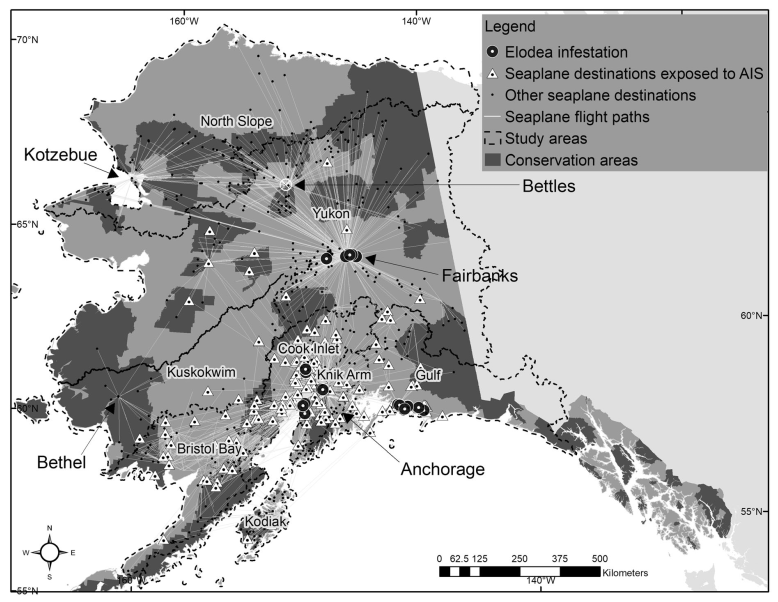
\includegraphics[width=0.75\linewidth]{tobymap.png}
                \caption{Map from "Flight plan for the future"}
                \label{fig:tobymap}
            \end{figure}



            \begin{figure}
                \centering
                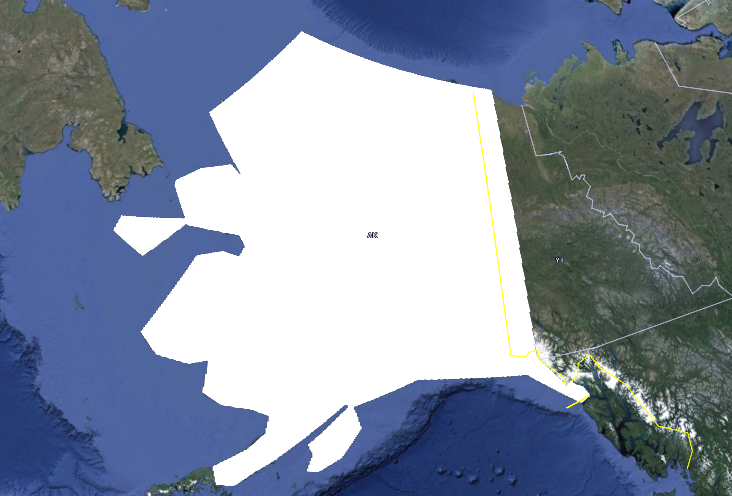
\includegraphics[width=0.75\linewidth]{polyimage.png}
                \caption{Proposed Polygon Visualized in Google Earth}
                \label{fig:akpoly}
            \end{figure}

            \begin{figure}
                \centering
                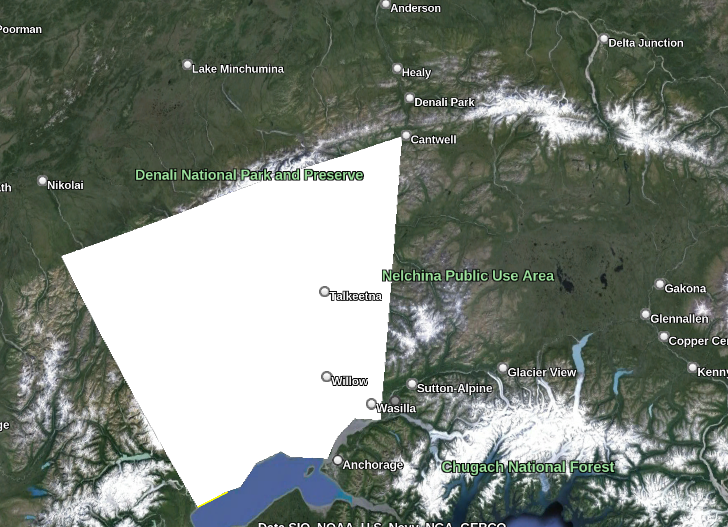
\includegraphics[width=0.75\linewidth]{susitnaroi.png}
                \caption{Backup Polygon if The Initial ROI is too Large}
                \label{fig:susitna}
            \end{figure}
            

        \section{Justification}

            During my research for my thesis, I have not been able to find very many papers or articles about which lakes are potentially "floatplane" accessible.  There is a fantastic report from the BLM \cite{trammel2016} that has tried to quantify this variable for the Central Yukon Region, and another excellent paper where a survey of floatplane pilots was conducted \cite{schwoerer2022flight} which identified 682 known floatplane destinations, and there are numerous papers about detecting new lakes \cite{zhang2014lakes}, or monitoring lake area or even volume by satellite \cite{sima2013using}.  However, I have not seen much information about simply counting lakes by shape.

            Given that my research is directly concerned with the transmission of an invasive species on aircraft floats, having a mapping of waterbodies that are "floatplane accessible" would be helpful for future monitoring and mitigation strategies.  Simply being able to rule out certain waterbodies for survey could have major practical benefits.  If you cannot get there by boat, or floatplane, then monitoring the lake for infestations probably isn't necessary. There are multiple other potential benefits to attempting to count the number of lakes that can be reached by float equipped aircraft as well.

            Float equipped fixed-wing aircraft add a lot of economic value to the state of Alaska.  The one study I found about floatplane based tourism in Alaska was from 2007, but it estimated approximately a quarter million dollars in revenue per season just to Chichagof Island from Juneau \cite{dugan2007nature} excluding lodge flights.  Identifying potentially "unexplored" lakes could be financially beneficial to local air carriers developing packages to explore remote parts of Alaska.
            
            Similarly, because float equipped airplanes are typically significantly cheaper to operate than helicopters with similar payloads identifying locations close to resource extraction projects could provide significant cost savings or even reduce the environmental impact of building a runway for exploratory projects.  If this can be done for Alaska, it can be done in other locations worldwide.

            The ability to measure the geometry of lakes or other waterbodies has a lot of practical application in other types of research.  While I do not claim to be a hydrologist, the shape and contours of lakes and rivers are key to analyzing topics in natural resource management, environmental studies, and computational geometry.  If we can narrow down the count of lakes by their shape and geometry, that will be applicable to many other tasks where the shape of the object that is sensed remotely is important.

            Finally, given the notable lack of papers on this topic specifically (really only one or two), I believe this is an opportunity to conduct truly novel research on a topic that is simultaneously approachable and interesting.  Beyond the economic and cross-disciplinary reasons, floatplanes are "cool" aviation is "fun" and exploring remote parts of Alaska is enjoyable.  This study will allow us to conduct truly novel research while exploring an interesting topic.

                
                

        \section{Workload and Analysis Division}


            I propose we split the analysis required by this project into several distinct components.

            \begin{enumerate}
                \item Lake Identification.  Someone needs to develop the appropriate skills to determine when a waterbody is a lake, and when it is something else entirely.  Swamps are not adequate for floatplane usage, but also visually, a lake that is covered in lilly-pads may not even appear to be a lake in the visual range, but might stand out some other way.  One of the group members is going to need to become the "lake" expert and be able to explain to the rest of us what is classified as a lake and how to measure them.

                \item Lake data extraction.  Someone needs to determine what characteristics make a lake "float plane accessible" (I can help with this), and then figure out how we can measure those characteristics (if we can) in Google Earth Engine in a way that is replicable.  We should be able to use data from the BLM study \cite{trammel2016} or the "Flight plan for the future" \cite{schwoerer2022flight} as a source of truth, but we should also search for more.

                \item Data Visualization.  It is not enough for us to simply identify the lakes in a spreadsheet collated by latitude and longitude.  The final project should involve exploration of the Google Earth Engine API to build a tool that we could display on a website.  If we can do that, I can host the website the finished product.

                \item Project Writeup and DevOps.  If we are able to get our project to work, we need to be able to share this information and we need to have decent test cases to ensure the code we write and our analyses are correct.  Naturally, we will have to present this project to the class so this part is cruicial, but also, we should start start looking for journals to publish this in over the summer.  If we have an extra person, it would be nice to have a person who's sole goal in life is to document, and figure out how to break our code, but if we have a team of three it will be all of our responsibility to fill this role.
            \end{enumerate}
                
                % ##########################################

            \section{Datasets and Thoughts on Data}

                Presently, I propose using LandSat and Sentinel-2 satellite data for this analysis.  If I was attempting to apply this research in the lower 48, I might use the LandSat data as well as  \href{https://www.arcgis.com/home/item.html?id=f1f45a3ba37a4f03a5f48d7454e4b654}{the National Hydrography Dataset Plus High Resolution} which appears to be updated frequently, however, this dataset may not include data in Alaska (though the map seems to indicate it does contain most of Alaska).  That dataset is a potential tool, but we will have to learn how to use it.
                
                For this study, we should be able to get by with the LandSat Surface Reflectance and/or the Top of Atmosphere data contained in the "Thematic Mapper" but the Sentinel-2 platform appears to have some resources that we cannot ignore.  The amazing github page \href{https://github.com/awesome-spectral-indices/awesome-spectral-indices}{about awesome spectral indices} seems to suggest that the NDWI (Normalized Difference Water Index), SWI (Sentinal Water Index), the SWM (Sentinel Water Mask), and a wide variety of other tools may help us identify waterbodies.  We should have ample data with either platform.  There appears to be a lot of research out of China presently on using this data for identifying waterbodies, the field appears to be evolving rapidly, but the Sentinel Water Index appears particularly effective in differentiating between "water" and "not water" \cite{jiang2021effective}.  According to the Sentinel-2 web page, we should have access to all of Alaska for these purposes, however, weather may limit use.
                
                The LandSat data is at 30m/px resolution and is likely sufficient, 30 meters even at the equator is slightly less than 100'.  In my experience, most pilots (even experienced bush pilots) are not accurate enough to fly to lakes or runways where the margins are that tight.  Given that we'll probably work with Sentinel-2 data initially, the resolution should be more than enough.  We can acquire source of truth data is available from the relevant papers.

            \section{Projections}

                LandSat data comes in a complicated projection called the "SOM" projection, or \href{https://landsat.gsfc.nasa.gov/about/space-oblique-mercator-projection/}{"Space Oblique Mercator"} and is translated to UTM (Universal Transverse Mercator).  Sentinel-2 data comes in the \href{https://www.sentinel-hub.com/faq/which-projection-best-exporting-data/}{UTM format}, the ellipsoid, if relevant appears to be WGS84 for both applications.

                This probably does not actually matter for our applications however.  Google Earth Engine displays in the mercator projection, which appears to be the same as the data coming from the source.  \href{https://developers.google.com/earth-engine/guides/projections}{More information available in the documentation here.}

                
        
        \section{References}

            By the time this is done, this will no-doubt be much longer - if we get 4 students for the project, I propose that the scribe maintain the references in in "bibtex" format for ease of use.  
        
            \bibliographystyle{plainnat}
            \bibliography{bibliography}

\end{document}